\documentclass[25pt, a0paper, landscape]{tikzposter}

% Packages required for tikzposter class
\usepackage{tikz, calc, ifthen, ae, xstring, etoolbox, xkeyval}
\usepackage{amsmath}
\usepackage{hyperref}
\usepackage{graphicx}
\usepackage{biblatex}

\addbibresource{draft.bib}

\definelayouttheme{Stankus}{
    \usecolorstyle[colorPalette=GreenGrayViolet]{Australia}
    \usebackgroundstyle{Default}
    \usetitlestyle{Empty}
    \useblockstyle{Basic}
    \useinnerblockstyle{Default}
    \usenotestyle{Default}
}

\usetheme{Stankus}
% turns off the comment on how the poster was created in the lower right corner of the poster
\tikzposterlatexaffectionproofoff

% How can we remove the white bar at the top of the poster?
% \titlegraphic{Logo}

\title{Recognizing Overlapping Handwritten Digits Using Neural Networks}
\institute{Frost Research 2018}
\author{Professor Mark Stankus\textsuperscript{*}, Alexa White\textsuperscript{*}, Cameron Fredrickson\textsuperscript{*}, Grant Bernosky\textsuperscript{*}, and Tim Royston\textsuperscript{*}}

\begin{document}
    \maketitle
    \begin{columns}
        \column{0.35}
        \block{Our Goal
        }{
            We wanted to use a machine learning concept called a neural network to learn
            how to identify handwritten overlapping and non overlapping digits to a high degree of accuracy.
            % image of a '4', a nonoverlapping '42', and a overlapping 58
            \begin{center}
                
\includegraphics[scale=6.0]{4.png}
                
\includegraphics[scale=6.0]{42.png}
                
\includegraphics[scale=6.0]{58.png}
            \end{center}
        }
        \block{What is a neural network made of?
        }{
            A neuron is a real-valued function which takes as input a vector $\mathbf{x}$,
            a vector of weights $\mathbf{w}$ and a bias $b$ which outputs $\sigma(\mathbf{x}\bullet\mathbf{w}+b)$.
            The function $\sigma$ is called an activation function whose output is usually within $[-1,1]$ or $[0,1]$.
            A commonly used activation function with a range of $[0,1]$ is the sigmoid function:
            \[
                \sigma(z) = \frac{1}{1+e^{-z}} \, .
            \]

            A densely-connected layer of neurons is a function which encapsulates a finite 
            number of neurons, where each neuron in the layer is connected to every neuron
            in the next layer.

            % neural network image
            \begin{center}
                \input{simplenn.input}
            \end{center}

            A layer is a vector-valued function which takes as input a vector $\mathbf{x}$, 
            a set of weight vectors $\mathbf{w_1},\ldots,\mathbf{w_m}$ and a set of biases 
            $b_1,\ldots,b_m$ which outputs 
            \[
                \begin{bmatrix}
                    \sigma(\mathbf{x}\bullet\mathbf{w_1}+b_1)\\
                    \vdots\\
                    \sigma(\mathbf{x}\bullet\mathbf{w_m}+b_m)\\
                \end{bmatrix}
            \]
        }
        \block{Cost Function for Classifying Single Digits
        }{
            \begin{itemize}
                \item A neural network used to classify single digit images 
                has an output vector $\mathbf{\hat{y}}_0$ with 10 entries.
                Each entry is a value between 0 and 1 and can be interpreted 
                as a probability that the given image is of a particular digit.
                The 1st entry corresponds to a '0', the 2nd entry to a '1' and 
                the 10th entry to a '9'.
                \bigskip
                
                \item For example, we might have
                $\mathbf{\hat{y}}_0 = [ 0 \ \  0 \ \  0 \ \  0.2 \ \  0.5 \ \  0.1 \ \  0.1 \ \  0 \ \  0 \ \  0 \ \  0]^T$.
                \bigskip

                \item Suppose the weights and biases of our neural network
                are $\mathbf{w}_0$ and $\mathbf{b}_0$
                and $\mathbf{x}_0$ is an image of a `4'.
                The label of $\mathbf{x}_0$ would be 
                $\mathbf{y}_0 = 
                [ 0 \ \  0 \ \  0 \ \  0 \ \  1 \ \  0 \ \ 0 \ \ 0 \ \ 0 \ \ 0 \ \ 0]^T$.
                \bigskip

                \item The cost function $C$ describes
                how close our prediction is to the label of the image
                and is defined by 
                \(
                    C_{\mathbf{x}_0} (\mathbf{w}_0,\mathbf{b}_0) 
                    =
                    \|\mathbf{y}_0-\mathbf{\hat{y}}_0\|
                \).
            \end{itemize}
        }
        \column{0.35}
        \block{How does a network learn?
        }{
            \begin{itemize}
                \item For a fixed $\mathbf{x}$, the graph of the function 
                    $C_{\mathbf{x}}$ is a surface
                \item To train a neural network we want to go ``downhill'' along that surface
                by following the negative of the gradient of $C_{\mathbf x}$
                \item We want to find $\mathbf{w}_0$ and $\mathbf{b}_0$ so that 
                    $C_{\mathbf{x}}(\mathbf{w}_0,\mathbf{b}_0)$
                    is small for each training vector $\mathbf{x}_0$
                \item The neural network ``has learned''
                    if $C_{\mathbf{x}}(\mathbf{w}_0,\mathbf{b}_0)$
                    is also small for each test vector $\mathbf{x}$
            \end{itemize}
        }
        \block{Training a Neural Network
        }{
            \begin{enumerate}
                \item Convert black and white images to matrices of $0$'s and $1$'s, then flatten them into vectors 
                \item Separate theses flattened vectors into training, validataion, and testing data
                \item Adjust the weights and biases as the training data is fed to the the neural network
                \item Validate those adjustments by testing the network on the validation data
                \item Train on several epochs, completing steps 3 and 4 is refered to as ``1 epoch''
                \item Feed in the test data to see how well the training generalizes
                    to unseen data.
                \item Save the neural network (the adjusted weights and biases)
                \item Now we can use the trained network to classify future data
            \end{enumerate}
        }
        \block{Image Recognition Solutions
        }{
            % The capsule network will predict the existence of a face if and
            % only if the mouth prediction of the face, the eye prediction of the face,
            % and the rest of the features all have the same prediction for the 
            % location and orientation of the entire face.

            % The capsule network will predict the location of the mouth and then
            % predict the location of the face based on the location and orientation
            % of the mouth

            Before 2017, the most common type of neural network used in image recognition
            was the convolutional neural network (cnn). A cnn 
            classifies images by determining the existence of 
            \textbf{certain features} in an image. 
            It does not consider the relative positions and orientations of these features.
            A cnn might recognize a nose, an eye, or a mouth, but classify both
            of the following as faces.
            \begin{center}
                \cite{pechyonkin_2017}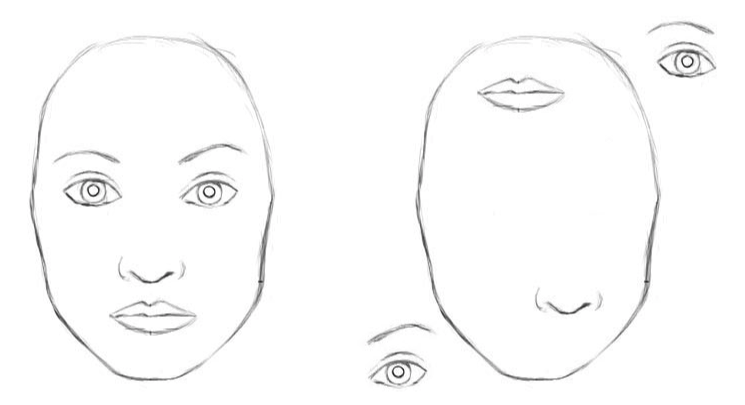
\includegraphics[scale=0.5]{cnn_problem.png}
            \end{center}
            A capsule network 
            \cite{NIPS2017_6975} 
            classifies an image as a face if and only if 
            positions and orientations of the the features relative to the 
            location of the face are correct.
            In the picture below on the right, recognizing the mouth would lead the network 
            to predict that the rest of the face would resemble the highest of 
            the three faces shown and recognizing the eye would lead the network 
            to predict that the rest of the face would resemble the lowest of 
            the three faces shown. Since the face predictions do not agree,
            the image is not classified as a face. 
            \begin{center}
                \cite{bourdakos_2018}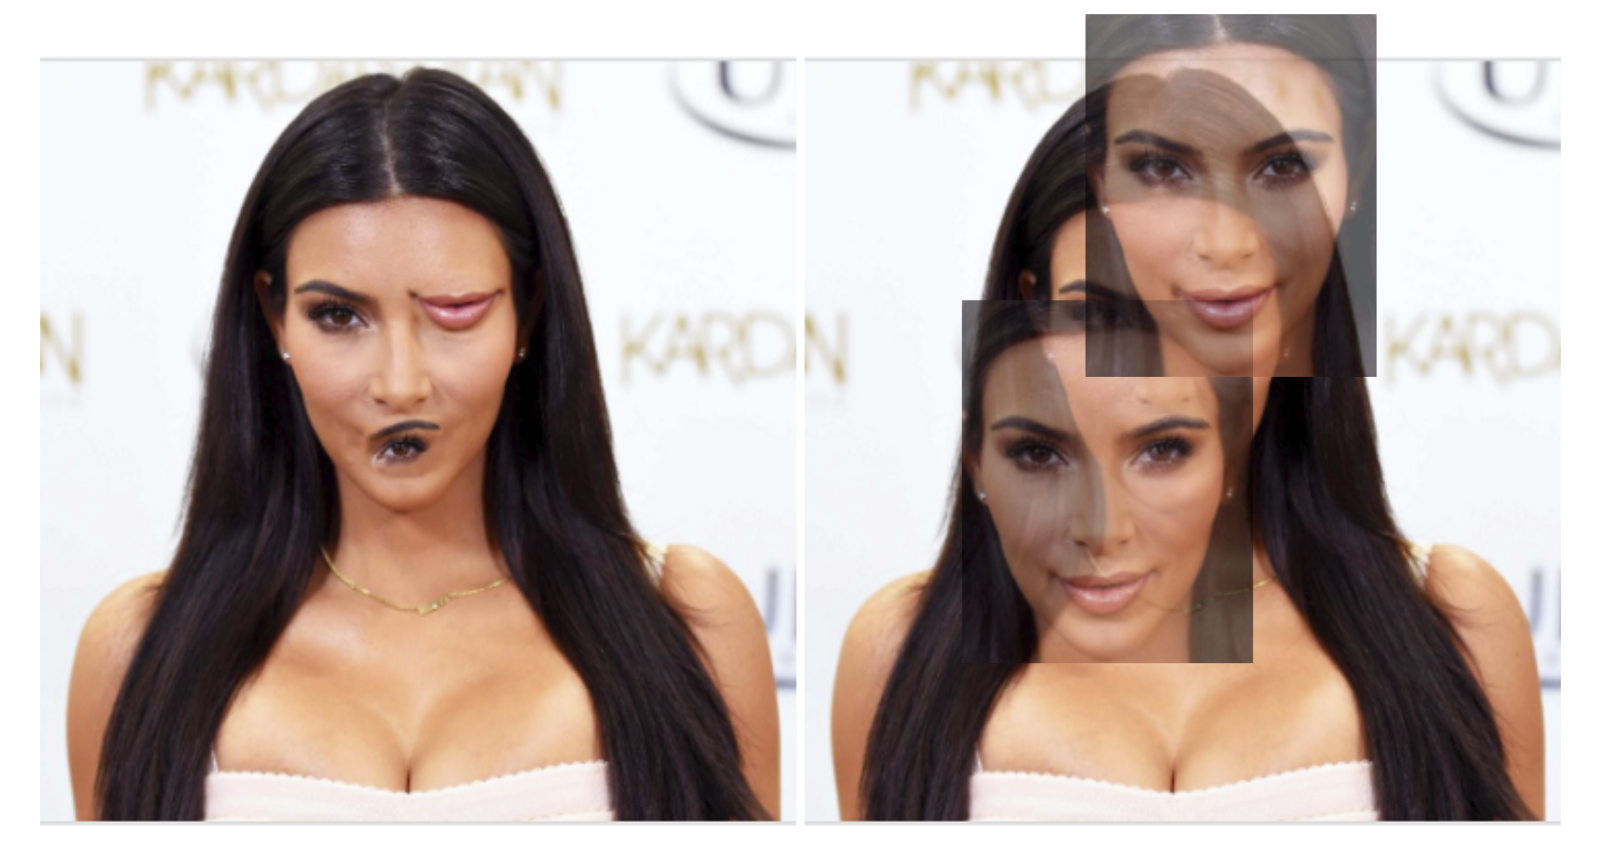
\includegraphics[scale=0.3]{capsule_network_solution.png}
            \end{center}
        }
        \column{0.3}
        \block{Our Solution
        }{
            {\Large\underline{\textbf{Our Data:}}}
            \begin{itemize}
                \item MNIST is a collection of single digit handwritten numbers. 
                \item With Python code and MNIST we created a dataset of single 
                    digit and overlapping double digit images.
            \end{itemize}

            {\Large\underline{\textbf{Our Neural Networks:}}}
            \begin{itemize}
                \item We used TensorFlow an open source machine learning framework
                    created by Google to code our neural networks.
                \item We created and trained a densely connected neural network
                    called choice\_net to classify each data sample in our randomly 
                    shuffled dataset as a single digit or double digit image
                \item The output of choice\_net is fed to one of 2 capsule 
                    networks named single\_caps and double\_caps which were 
                    trained on single digit and double digit images respectively.
            \end{itemize}
        }
        \block{Results
        }{
            All of our neural networks were trained on 2 epochs of 60,000 training samples and
            5,000 validation samples. Our testing dataset contained 10,000 samples.

            \begin{itemize}
                \item choice\_net achieved a test accuracy of 99.9+\%
                \item The single\_digit\_caps achieved a test accuracy of 99.1987\%
                \item The double\_digit\_caps achieved a test accuracy of 98.8381\%
            \end{itemize}
            The code is publically available at
            \url{https://github.com/mstankus/Frost-Neural-Network-Research-2018}.
        }
        \block{References
        }{
            \printbibliography[heading=none]
            (This is a partial list containing the resources used to create the poster)
        }
        \block{Acknowledgments
        }{
            \textsuperscript{*} Frost Research Fellows, funded by the Bill and Linda Frost Fund, Cal Poly, San Luis Obispo
        }
    \end{columns}
\end{document}
